Process aware information systems (PAIS) are becoming more and more widespread. These information systems log huge amounts of events, and even more event data can be extracted from all other kinds of ubiquitous organizational databases \cite{van2015extracting}.
Additionally, in our increasingly digitized world, not just business processes are being recorded. Social media, smartphone sensors (e.g. location) and medical devices are just some of the other possible sources of event data.
The goal of process mining is to exploit these masses of event data to answer two types of fundamental questions regarding the process behind the data.
\begin{enumerate}
    \item \emph{Conformance} \textemdash \ in what way does the observed behavior deviate from the norm? Are rules and regulations being followed?
    \item \emph{Performance} \textemdash \ how long do certain tasks take? What are the bottlenecks?
\end{enumerate}
A prerequisite to answering these questions is to have a process model to compare the data to.
Models which describe the way the process \emph{should} be performed are called \emph{de jure} models. They can be hand-made and exist separately from the observed data. If such a model does not exist, approaches using the mechanism \emph{discovery} are used to create so-called \emph{de facto} models which are solely based on the observed data.
Handling noise, incompleteness and Big Data is part of ongoing research for improving this mechanism.
Figure \ref{fig:procapproaches} also shows the other mechanism \emph{replay} which confronts the given log with a given or discovered model. Approaches using this mechanism can create all kinds of diagnostics like metrics, descriptions or enriched models. Enriching a model entails projecting useful information, extracted from the data, on the structure of the model, e.g. marking where deviations take place.
\begin{figure}
    \centering
    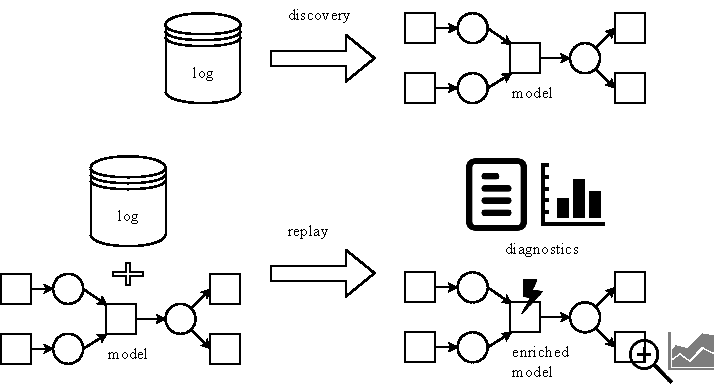
\includegraphics{figures/introduction/activities_schematic.pdf}
    \caption{Process mining mechanisms}
    \label{fig:procapproaches}
\end{figure}

This enables insights into different perspectives on the two fundamental questions.
We focus on the notion of \emph{fitness} for conformance and \emph{throughput} for performance.
Fitness measures how well the model is able to mimic the observed behavior. This in turn can be used to detect where behavior occurred in reality that was not intended. Throughput ranges from case duration to waiting times between events.
The influence of \emph{data} attributes, like who executed an event, and \emph{process context} is considered as well.
Process context ranges from local, like how many cases are currently active (busyness), to external like the weather. We only measure the local process context in the form of busyness here since external context is almost impossible to handle.

A shortcoming of state-of-the-art approaches is that they often give overall results and averages. For example, one fitness value for the entire log and model. This is useful for determining if a model has sufficient fitness but not for finding out where the deviations take place. Even more important is the fact that real-life processes are often dynamic and change in some way over time which is called concept drift. That means a low fitness or bad throughput may indicate that the process was always this way or that it behaved perfectly for the first part of the observed timeframe and only got worse after that. Additionally, even the correlations between several measured aspects may be variable over time. A low fitness could lead to bad performance, but this might also reverse.

As an example, consider the Petri net model given in Figure \ref{fig:bigschematic}. It describes the control-flow of a small credit application process where every application starts with a submission. Then, the credit history of the applicant is checked. If the result is \emph{OK}, the application should be accepted and otherwise rejected. After accepting, the credit is provisioned, and the payment is setup concurrently. Finally, the credit is sent. The information system logs the credit amount for cases, time and type of activity for events but no resource information.

However, in real-life, a certain employee is not following protocol. Whenever the load at his position is high and no one notices, he simply accepts low value applications where the credit history check was negative. Additionally, he actively delays high value applications, making them wait for acceptance longer. All of this only happens for a short part of the whole logged time span.

To discover such a complex pattern in full detail in the event data given the model, multiple perspectives are necessary. More specifically,
\begin{itemize}
    \item \emph{Fitness} \textemdash \ Applications which should be rejected are accepted
    \item \emph{Throughput} \textemdash \ Applications are being delayed
    \item \emph{Data} \textemdash \ Only low value applications deviate, and only high value applications are delayed
    \item \emph{Process Context} (local) \textemdash \ All of this only happens when the affected places are busy, i.e. many cases are currently waiting there
\end{itemize}
Condensing the perspectives into single results would obscure the entire pattern. The fitness would still be near perfect, since only specific cases deviate and only during a certain short timeframe. This is also true for the other perspectives.
As a first step, as shown in the overview of our approach in Figure \ref{fig:bigschematic}, we localize the perspectives over \emph{control-flow}. That means we can now differentiate the stages of the process. This allows us to detect a stronger deviation on the place after \textsc{Check\_NOK} and longer throughput times on the place after \textsc{Check\_OK}.
However, averaging over the whole timespan would still not allow us to find out when it happened.
The next step is localizing over \emph{time}, leading to the goal of having a timeseries for each place of the model. These finally make it possible to fully discover the problematic pattern described above.

The example shows that averaging, especially over time, can make it impossible to detect complex patterns in event logs. To solve this problem, we propose localizing conformance and performance over control-flow by considering each place individually and then localizing it further over time by discretizing the process duration.

\begin{figure}
    \centering
    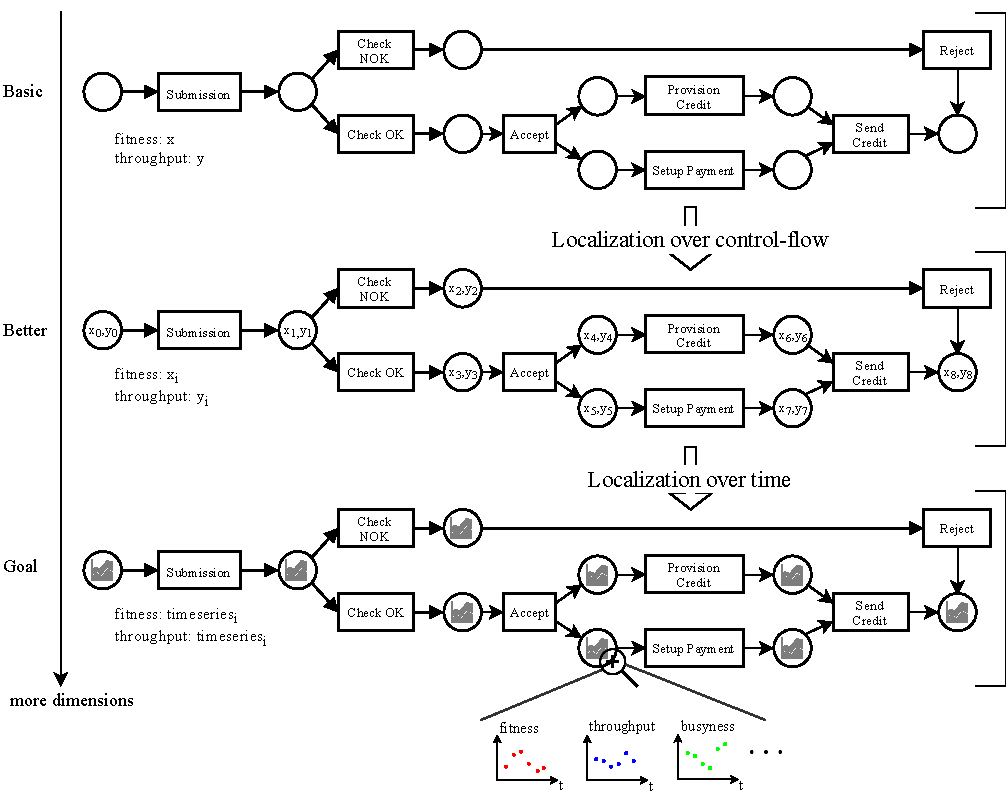
\includegraphics[width=\textwidth]{figures/introduction/bigschematic.pdf}
    \caption{Overview of the approach}
    \label{fig:bigschematic}
\end{figure}

Chapter \ref{chap:prelim} covers the preliminaries necessary for our work. In Chapter \ref{chap:appr}, we present our approach. Following that, the implementation in ProM is detailed in Chapter \ref{chap:impl}. Then, the approach is evaluated on synthetic and real-life event logs in Chapter \ref{chap:eval}. Second to last, related work is discussed in Chapter \ref{chap:related} and the report is concluded in Chapter \ref{chap:conclusion}.